\chapter{Fotosynthese}\label{ch:g12:photosynthesis}

Zet een takje waterpest ondersteboven in een pot water onder een lamp, en
er stijgt een stroom belletjes op uit de afgesneden steel: zuurstof, om de
paar seconden een belletje, sneller als de lamp dichterbij wordt gebracht,
en gestopt zodra hij uitgaat. Het gas is de zichtbare helft van een proces
dat elk dier op de planeet voedt en dat de lucht twee miljard jaar geleden
adembaar heeft gemaakt. \cref{ch:g10:cell-metabolism} gaf het in één
regel: koolstofdioxide en water worden, met licht, suiker en zuurstof. Dit
hoofdstuk opent de \omterm{def:g12:photosynthesis:chloroplast}{bladgroenkorrel} en volgt de energie van een foton tot
in een chemische binding.

\section{De bladgroenkorrel}

\begin{definition}[Bladgroenkorrel]\label{def:g12:photosynthesis:chloroplast}
De \emph{bladgroenkorrel}\index{bladgroenkorrel} is het \omterm{def:g10:cells-common-unit:organelle}{organel} van de
\omterm{def:g10:cell-metabolism:autotrophy}{fotosynthese}: een lensvormig lichaampje van zo'n \qty{5}{\micro m} lang,
begrensd door een dubbel membraan, met daarin een vloeistof, het
\emph{stroma}, waarin stapels afgeplatte membraanzakjes liggen, de
\emph{thylakoïden}\index{thylakoïde}. De thylakoïdemembranen dragen de
kleurstoffen --- \emph{chlorofyl} a en b, groen, en oranje carotenoïden
--- en de \omterm{def:g10:chemistry-of-life:families}{eiwitten} die lichtenergie omzetten; het stroma draagt de \omterm{def:g11:enzymes-and-phenotype:enzyme}{enzymen}
die suiker bouwen. Een bladcel bevat tientallen \omterm{def:g10:cells-common-unit:organelle}{bladgroenkorrels}, een
vierkante millimeter blad zo'n half miljoen.
\end{definition}

\begin{omfigure}
\begin{tikzpicture}
  \node[anchor=south west, inner sep=0] (img) at (0,0)
    {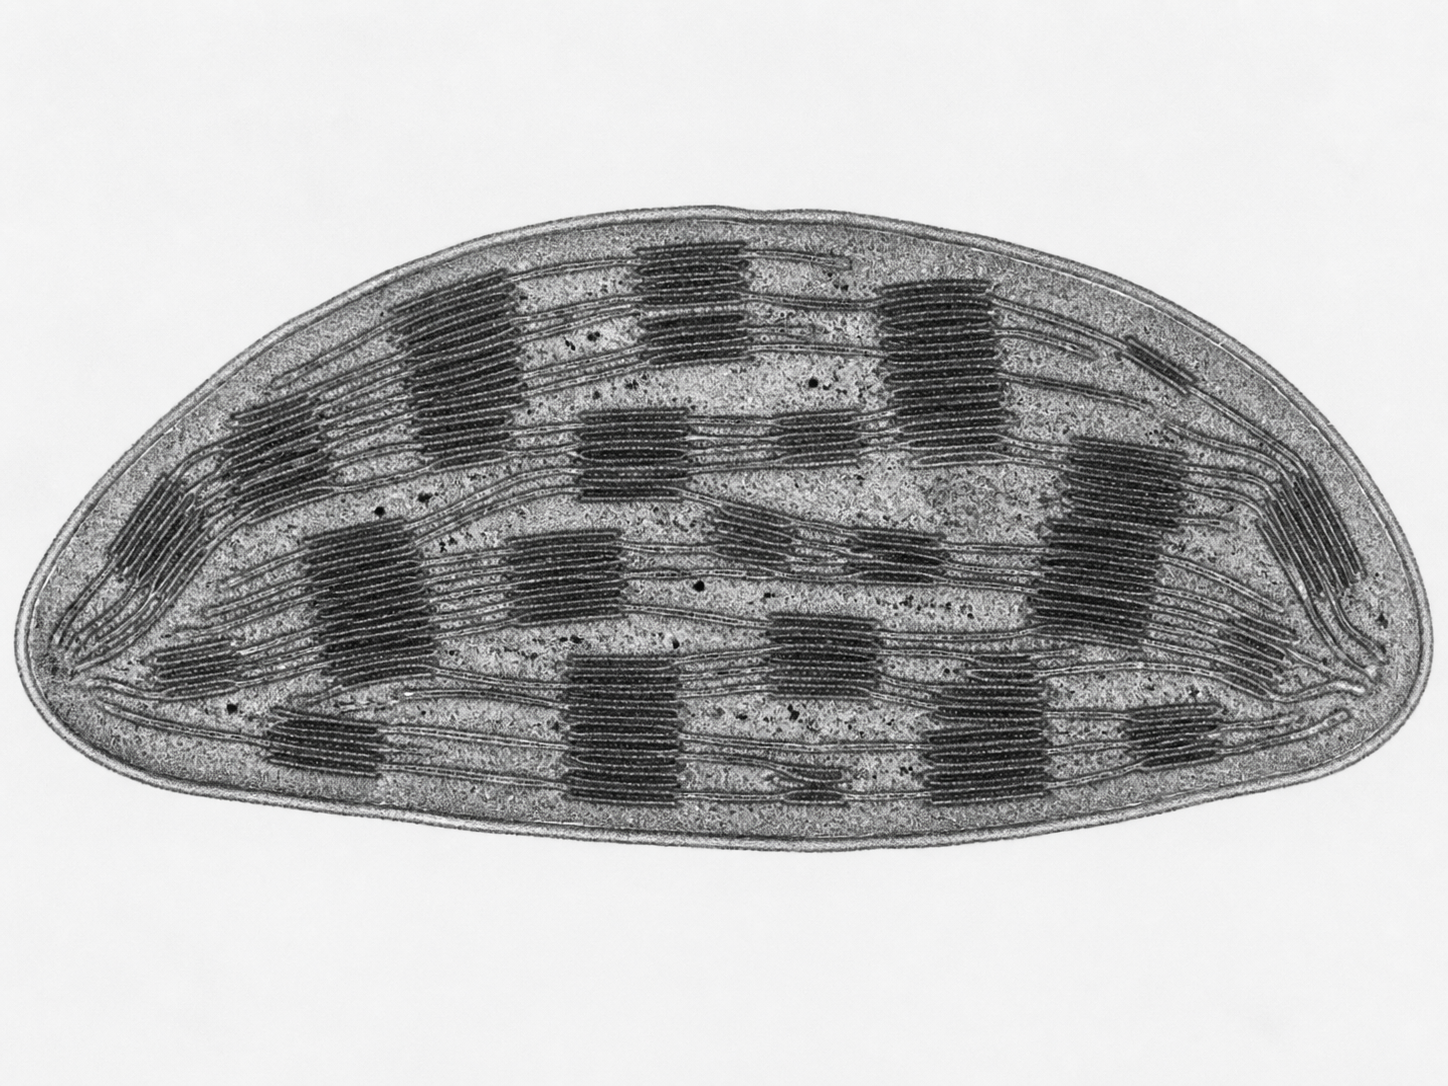
\includegraphics[width=0.5\linewidth]{images/book2/ai/g12-photo-chloroplast-tem.png}};
  \begin{scope}[x={(img.south east)}, y={(img.north west)},
      every node/.style={font=\small}]
    \draw[omDef, thick] (0.10,0.50) -- (-0.04,0.80) node[left, align=right] {dubbele\\ envelop};
    \draw[omDef, thick] (0.47,0.72) -- (0.47,1.06) node[above] {gestapelde thylakoïden (een granum)};
    \draw[omDef, thick] (0.62,0.42) -- (1.04,0.20) node[right] {stroma};
    \draw[omDef, thick] (0.80,0.60) -- (1.04,0.75) node[right, align=left] {membranen die de\\ stapels verbinden};
  \end{scope}
\end{tikzpicture}

{\small Een \omterm{def:g12:photosynthesis:chloroplast}{bladgroenkorrel} in de elektronenmicroscoop: de dubbele
envelop, het stroma, en de thylakoïdemembranen gestapeld tot grana, waar
de kleurstoffen zitten. Het licht wordt in de membranen opgevangen; de
suiker wordt gebouwd in de vloeistof eromheen.}
\end{omfigure}

\begin{proposition}[Welk licht wordt gebruikt]\label{prop:g12:photosynthesis:spectrum}
Chlorofyl neemt blauw en rood licht sterk op en groen licht vrijwel niet
--- en daarom zijn bladeren groen. De \omterm{def:g10:cell-metabolism:autotrophy}{fotosynthese} wordt aangedreven door
de golflengtes die de kleurstoffen opnemen: tegen de golflengte uitgezet
stijgt en daalt haar snelheid (het \emph{werkingsspectrum}) met de
opname door de kleurstoffen, met toppen in het blauw en het rood en een
dal in het groen.
\end{proposition}
\begin{proof}[Bewijsmateriaal]
Engelmann (1882) legde een draad groenwier in een druppel water met
bacteriën die naar zuurstof toe zwemmen, en projecteerde door de
microscoop een spectrum langs de draad: de bacteriën verzamelden zich rond
de stukken die in het blauw en het rood werden belicht, en meden het groen
--- daar waar die kleuren vielen, kwam zuurstof vrij. Een moderne meting
van de zuurstofafgifte onder gekleurde lampen geeft dezelfde kromme, en
die valt samen met het opnamespectrum van de eruit gehaalde kleurstoffen.
\end{proof}

\begin{omfigure}
\begin{tikzpicture}
\begin{axis}[
  width=0.88\linewidth, height=5.8cm,
  axis x line=bottom, axis y line=left,
  xmin=400, xmax=700, ymin=0, ymax=110,
  xlabel={golflengte (nm)}, ylabel={\% van het maximum},
  xlabel style={font=\small, at={(axis description cs:0.5,-0.12)}, anchor=north},
  ylabel style={font=\small},
  tick label style={font=\small}, xtick={400,450,500,550,600,650,700}, ytick={0,50,100},
  legend style={at={(0.5,-0.3)}, anchor=north, legend columns=2, font=\small, draw=none},
]
\addplot[thick, omMeth, smooth] coordinates {(400,70) (430,100) (450,75) (480,35) (500,15) (550,8) (600,15) (640,45) (665,90) (680,70) (700,10)};
\addplot[thick, omThm, dashed, smooth] coordinates {(400,65) (430,85) (450,80) (480,55) (500,35) (550,25) (600,35) (640,60) (665,95) (680,100) (700,20)};
\legend{opname door de bladkleurstoffen, snelheid van de fotosynthese (werkingsspectrum)}
\end{axis}
\end{tikzpicture}

{\small De opname van licht door de uit een blad gehaalde kleurstoffen, en
de snelheid van de \omterm{def:g10:cell-metabolism:autotrophy}{fotosynthese} van het blad, tegen de golflengte. Beide
pieken in het blauw en het rood en zakken in het groen: het licht dat de
\omterm{def:g10:cell-metabolism:autotrophy}{fotosynthese} aandrijft is het licht dat de kleurstoffen opnemen.}
\end{omfigure}

\section{De lichtfase: water gesplitst, energie opgeslagen}

\begin{proposition}[Wat er in de thylakoïden gebeurt]\label{prop:g12:photosynthesis:lightphase}
In de thylakoïdemembranen gebeuren er in het licht drie dingen tegelijk:
\begin{itemize}
  \item watermoleculen worden \emph{gesplitst}: hun zuurstof komt vrij als
        $\mathrm{O_2}$ --- de zuurstof van de \omterm{def:g10:cell-metabolism:autotrophy}{fotosynthese} komt uit water
        en niet uit koolstofdioxide --- en hun waterstof wordt vastgehouden
        als elektronen en protonen;
  \item de energie van de opgenomen fotonen wordt gebruikt om die
        elektronen op een dragermolecule te laden, \emph{gereduceerd
        NADP}, dat het stroma als bron van waterstof zal gebruiken;
  \item dezelfde energie drijft de vorming van \emph{ATP} aan.
\end{itemize}
De lichtfase zet het licht dus om in twee chemische producten, ATP en
gereduceerd NADP, en geeft zuurstof af als bijproduct. Er komt geen
koolstofdioxide aan te pas.
\end{proposition}
\begin{proof}[Bewijsmateriaal]
Hill (1937) belichtte losgemaakte \omterm{def:g10:cells-common-unit:organelle}{bladgroenkorrels} in water met een
kunstmatige elektronenontvanger en zonder koolstofdioxide: zij gaven
zuurstof af en reduceerden de ontvanger. De afgifte van zuurstof heeft dus
licht en water nodig maar geen $\mathrm{CO_2}$, en is aan de overdracht
van elektronen gekoppeld. Ruben en Kamen (1941) gaven wieren water met de
zware isotoop $^{18}$O: de vrijgekomen zuurstof was zwaar; met zware
koolstofdioxide en gewoon water was zij dat niet. De zuurstof komt uit het
water.
\end{proof}

\begin{omfigure}
\begin{tikzpicture}[font=\small, >=Stealth,
  b/.style={draw, rounded corners, align=center, minimum height=1.0cm}]
  % thylakoid box
  \node[b, fill=omMeth!15, text width=3.6cm, minimum height=3.2cm] (thy) at (0,0) {};
  \node[anchor=north, font=\small\bfseries] at (thy.north) {thylakoïdemembranen};
  \node[font=\small, align=center] at (0,-0.1) {licht opgenomen\\ door chlorofyl};
  % stroma box
  \node[b, fill=omDef!10, text width=3.6cm, minimum height=3.2cm] (str) at (6.4,0) {};
  \node[anchor=north, font=\small\bfseries] at (str.north) {stroma};
  \node[font=\small, align=center] at (6.4,-0.1) {calvincyclus:\\ $\mathrm{CO_2}$ vastgelegd\\ in suiker};
  % inputs/outputs
  \draw[->, thick, omProp] (-3.2,1.0) -- (thy.west |- 0,1.0) node[pos=0, left, omProp] {licht};
  \draw[->, thick] (-3.2,-0.6) -- (thy.west |- 0,-0.6) node[pos=0, left] {$\mathrm{H_2O}$};
  \draw[->, thick] (thy.south) -- ++(0,-1.0) node[below] {$\mathrm{O_2}$ afgegeven};
  \draw[->, thick, omThm] (thy.east |- 0,0.7) -- (str.west |- 0,0.7) node[midway, above] {ATP};
  \draw[->, thick, omThm] (thy.east |- 0,-0.3) -- (str.west |- 0,-0.3) node[midway, above] {gereduceerd NADP};
  \draw[->, thick, gray] (str.west |- 0,-1.1) -- (thy.east |- 0,-1.1) node[midway, below, font=\scriptsize] {dragers keren terug};
  \draw[->, thick] (9.6,0.6) -- (str.east |- 0,0.6) node[pos=0, right] {$\mathrm{CO_2}$};
  \draw[->, thick] (str.east |- 0,-0.6) -- (9.6,-0.6) node[right] {suiker};
\end{tikzpicture}

{\small De twee fasen van de \omterm{def:g10:cell-metabolism:autotrophy}{fotosynthese}. In de thylakoïdemembranen
splitst het licht water, geeft het zuurstof af en laadt het twee dragers,
ATP en gereduceerd NADP. In het stroma betalen die dragers het vastleggen
van koolstofdioxide in suiker. De eerste fase heeft licht nodig; de tweede
alleen haar producten.}
\end{omfigure}

\section{De koolstoffase: suiker gebouwd}

\begin{proposition}[De calvincyclus]\label{prop:g12:photosynthesis:calvin}
In het stroma wordt koolstofdioxide, één molecule tegelijk, door het
overvloedigste \omterm{def:g11:enzymes-and-phenotype:enzyme}{enzym} op aarde gehecht aan een al aanwezige suiker met vijf
koolstofatomen; het product met zes koolstofatomen splitst meteen in twee
moleculen met drie koolstofatomen, die --- met de ATP en het gereduceerde
NADP van de lichtfase --- tot suikers met drie koolstofatomen worden
gereduceerd. De meeste daarvan worden hergebruikt om de ontvanger met vijf
koolstofatomen opnieuw te vormen, waarmee de \emph{calvincyclus}\index{calvincyclus}
sluit; één op de zes verlaat de cyclus als de nettowinst van de plant.
Drie rondes van de cyclus, drie $\mathrm{CO_2}$ vastgelegd, negen ATP en
zes gereduceerd NADP besteed: één uitgevoerde suiker met drie
koolstofatomen. Twee daarvan maken een glucose.
\end{proposition}
\begin{proof}[Bewijsmateriaal]
Calvin (jaren vijftig) gaf wieren enkele seconden lang koolstofdioxide
gemerkt met radioactief $^{14}$C, doodde hen in kokende alcohol en
scheidde hun moleculen: na vijf seconden zat het merk in één enkel zuur
met drie koolstofatomen; na dertig, in suikers met drie koolstofatomen en
in de ontvanger met vijf; na enkele minuten, in sacharose en zetmeel. Het
licht wegnemen liet de ontvanger onhervormd en het zuur met drie
koolstofatomen ophopen; de $\mathrm{CO_2}$ wegnemen liet de ontvanger
ophopen. De volgorde van verschijnen is de volgorde van de cyclus.
\end{proof}

\begin{omfigure}
\begin{tikzpicture}[font=\small, >=Stealth]
  \draw[thick, ->] (90:2.2) arc (90:-30:2.2);
  \draw[thick, ->] (-30:2.2) arc (-30:-150:2.2);
  \draw[thick, ->] (-150:2.2) arc (-150:-270:2.2);
  \node[draw, rounded corners, fill=omDef!12, align=center, font=\small] at (90:2.2) {ontvanger met\\ 5 C ($\times 3$)};
  \node[draw, rounded corners, fill=omProp!15, align=center, font=\small] at (-30:2.2) {zuur met 3 C\\ ($\times 6$)};
  \node[draw, rounded corners, fill=omMeth!15, align=center, font=\small] at (-150:2.2) {suiker met 3 C\\ ($\times 6$)};
  \draw[->, thick] (3.6,2.2) -- (2.4,1.6) node[pos=0, right, align=left] {$3\,\mathrm{CO_2}$ komen binnen};
  \draw[->, thick, omThm] (2.2,-2.4) -- (1.2,-2.0) node[pos=0, right, omThm, align=left] {6 ATP, 6 gereduceerd NADP\\ uit de lichtfase};
  \draw[->, thick, omThm] (-3.6,1.0) -- (-2.2,1.4) node[pos=0, left, omThm] {3 ATP};
  \draw[->, thick] (-2.4,-2.4) -- (-3.6,-3.2) node[anchor=north, align=center] {1 suiker met 3 C vertrekt:\\ een halve glucose};
  \node[font=\scriptsize, align=center] at (0,0) {5 van de 6 suikers\\ bouwen de\\ 3 ontvangers terug};
\end{tikzpicture}

{\small De \omterm{prop:g12:photosynthesis:calvin}{calvincyclus}, geteld over drie rondes. Drie koolstofdioxides
voegen zich bij drie ontvangers met vijf koolstofatomen; de zes producten
met drie koolstofatomen worden tot suikers gereduceerd ten koste van de
ATP en het gereduceerde NADP van de lichtfase; vijf van de zes worden tot
de ontvangers hergebruikt en één is de winst.}
\end{omfigure}

\begin{example}[De boekhouding van een glucose]\label{ex:g12:photosynthesis:bookkeeping}
Eén glucose heeft zes koolstofdioxides nodig, dus zes rondes van de
cyclus, 18 ATP en 12 gereduceerd NADP, allemaal geleverd door de
lichtfase, die daarvoor 12 watermoleculen splitst en zes zuurstoffen
afgeeft. Netto:
$6\,\mathrm{CO_2} + 12\,\mathrm{H_2O} \to \mathrm{C_6H_{12}O_6} +
6\,\mathrm{O_2} + 6\,\mathrm{H_2O}$ --- de samenvattende vergelijking van
\cref{ch:g10:cell-metabolism}, nu met het water aan beide kanten, omdat de
vrijgekomen zuurstof uit het gesplitste water komt en niet uit de
koolstofdioxide.
\end{example}

\begin{omfigure}
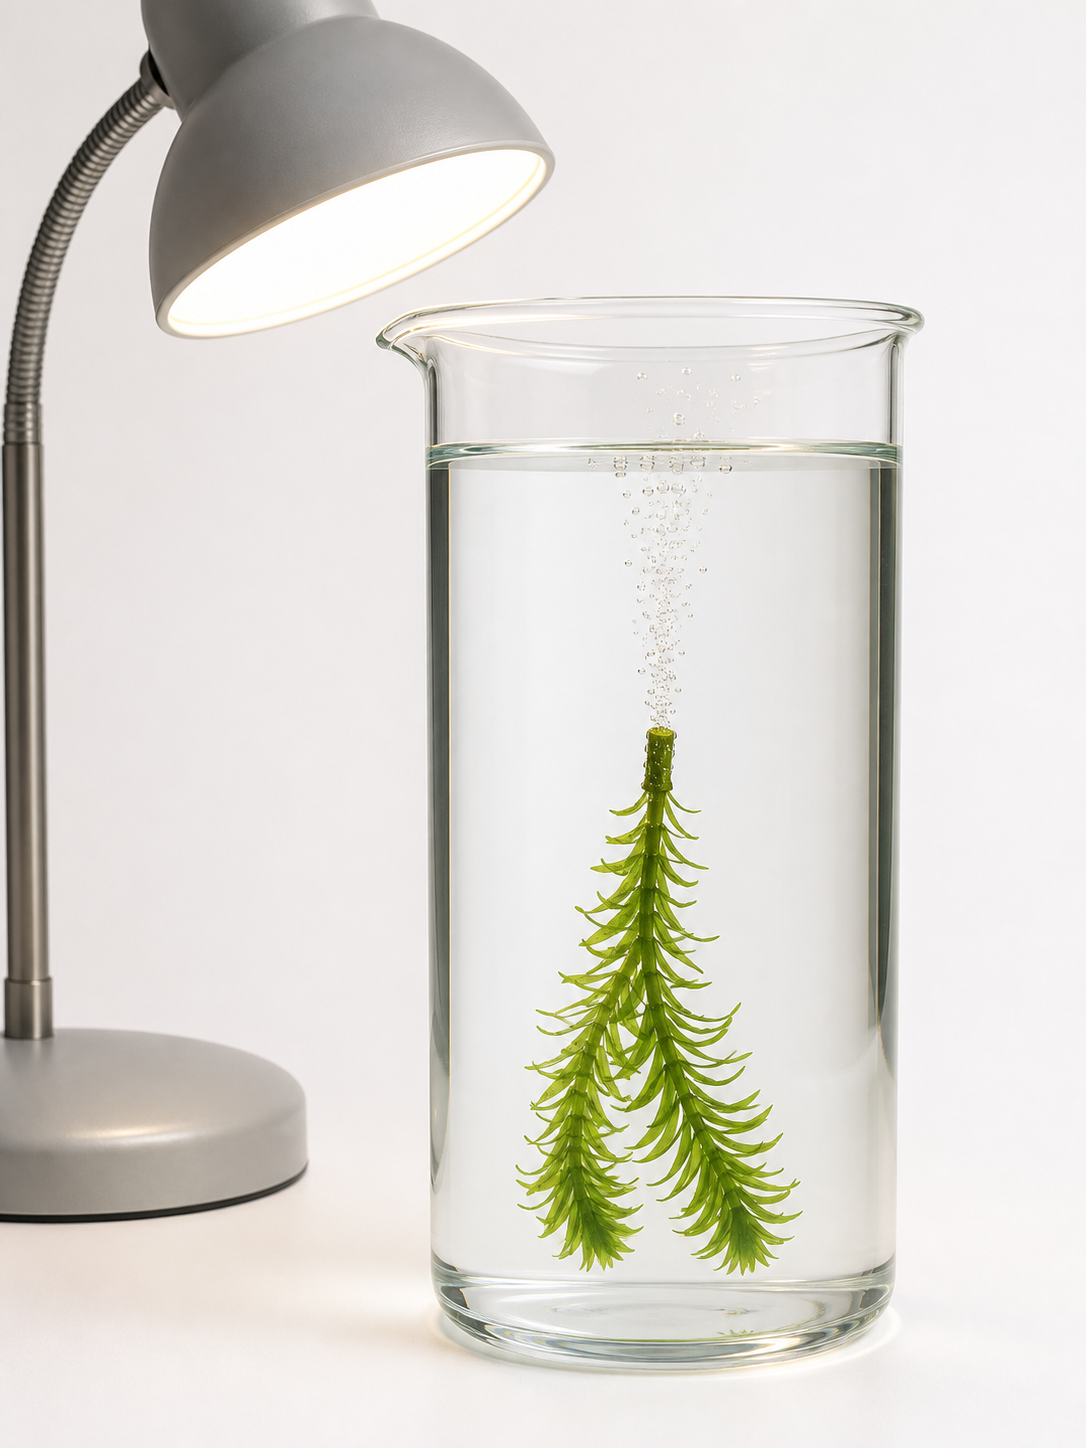
\includegraphics[width=0.34\linewidth]{images/book2/ai/g12-photo-elodea-bubbles.png}

{\small Waterpest onder een lamp: de belletjes die uit de afgesneden steel
opstijgen zijn de zuurstof van de lichtfase. Tel ze per minuut, verplaats
de lamp, verander haar kleur, en de snelheid van de \omterm{def:g10:cell-metabolism:autotrophy}{fotosynthese} is
gemeten.}
\end{omfigure}

\section{Wat de suiker wordt, en hoeveel er is}

\begin{proposition}[Bestemmingen van het product]\label{prop:g12:photosynthesis:fates}
De suikers met drie koolstofatomen die de cyclus verlaten, worden in de
\omterm{def:g12:photosynthesis:chloroplast}{bladgroenkorrel} samengevoegd tot \emph{zetmeel}, de dagvoorraad van het
blad, of naar het \omterm{def:g10:cells-common-unit:cell}{cytoplasma} uitgevoerd en in \emph{sacharose} omgezet, de
suiker die het \omterm{prop:g12:plant-rooted-life:saps}{floëem} vervoert (\cref{ch:g12:plant-rooted-life}). Daaruit
maakt de plant al het andere: cellulose voor wanden, vetten, en --- met
stikstof en zwavel uit de bodem --- \omterm{def:g10:chemistry-of-life:families}{aminozuren} en \omterm{def:g10:universal-dna:nucleotide}{nucleotiden}. De
\omterm{def:g10:cell-metabolism:autotrophy}{fotosynthese} is de bron van niet alleen de energie van de plant maar van
al haar \omterm{def:g10:chemistry-of-life:mineral-organic}{organische stof}, en, via de voedselketens, van vrijwel alle
\omterm{def:g10:chemistry-of-life:mineral-organic}{organische stof} op aarde.
\end{proposition}
\admitted

\begin{example}[Rendement, van blad tot planeet]\label{ex:g12:photosynthesis:efficiency}
Vol zonlicht levert ongeveer \qty{1000}{W} per vierkante meter, waarvan
zo'n 45\% in golflengtes ligt die de kleurstoffen kunnen gebruiken; een
blad zet daarvan overdag hoogstens zo'n 5\% om in suiker, en een gewas
over een seizoen 1\% tot 2\% van het totale zonlicht in biomassa. Hoe
klein dat deel ook is, de som is enorm: de \omterm{def:g10:cell-metabolism:autotrophy}{fotosynthese} legt ongeveer
\qty{1e11}{t} koolstof per jaar vast --- een zevende van de koolstof in de
dampkring --- en geeft de zuurstof af die de ademhaling, het vuur en de
roest verbruiken.
\end{example}

\begin{method}[Redeneren over een proef met fotosynthese]\label{met:g12:photosynthesis:experiment}
\begin{enumerate}
  \item Bepaal wat er wordt gemeten: afgegeven zuurstof (de lichtfase),
        opgenomen koolstofdioxide of gevormde suiker (de koolstoffase), of
        biomassa (alles, over de tijd).
  \item Bepaal wat er wordt gevarieerd: licht (sterkte, kleur),
        koolstofdioxide, temperatuur, water --- en op welke fase het
        inwerkt.
  \item Denk eraan dat de plant tegelijk ademt: een gemeten
        zuurstofafgifte is de productie min de ademhaling; in het donker
        is alleen de ademhaling te zien (\cref{ch:g10:cell-metabolism}).
  \item Volg de merken: $^{18}$O in water verschijnt in de zuurstof;
        $^{14}$C in koolstofdioxide verschijnt in de suikers, in de
        volgorde van de cyclus.
\end{enumerate}
\end{method}

\begin{remark}[Licht, en dan scheikunde]\label{rem:g12:photosynthesis:light}
De enige stap van de \omterm{def:g10:cell-metabolism:autotrophy}{fotosynthese} die licht nodig heeft, is de eerste: het
laden van elektronen uit water op een drager, met de afgifte van zuurstof.
Al het volgende --- het maken van ATP, het vastleggen van koolstofdioxide,
het bouwen van suiker --- is scheikunde die in het donker doorgaat zolang
de dragers strekken, en die de ademhaling van het volgende hoofdstuk
achterstevoren zal laten lopen. De \omterm{def:g12:photosynthesis:chloroplast}{bladgroenkorrel} is waar zonlicht in
chemische munt wordt omgezet; de rest van de \omterm{def:g10:cells-common-unit:cell}{cel}, en de rest van de
biosfeer, geeft haar uit.
\end{remark}

\section{Oefeningen}

\begin{exercise}[$\star$]\label{exo:g12:photosynthesis:1}
Beschrijf de \omterm{def:g12:photosynthesis:chloroplast}{bladgroenkorrel} en zeg waar de kleurstoffen zitten en waar de
\omterm{def:g11:enzymes-and-phenotype:enzyme}{enzymen} die suiker bouwen.
\end{exercise}

\begin{exercise}[$\star$]\label{exo:g12:photosynthesis:2}
Waarom zijn bladeren groen? Welke kleuren drijven de \omterm{def:g10:cell-metabolism:autotrophy}{fotosynthese} het best aan?
\end{exercise}

\begin{exercise}[$\star$]\label{exo:g12:photosynthesis:3}
Noem de drie producten van de lichtfase en zeg welk daarvan een bijproduct
is.
\end{exercise}

\begin{exercise}[$\star$]\label{exo:g12:photosynthesis:4}
Waar komt de zuurstof vandaan die een plant afgeeft, en hoe is dat
aangetoond?
\end{exercise}

\begin{exercise}[$\star$]\label{exo:g12:photosynthesis:5}
Hoeveel moleculen koolstofdioxide, hoeveel ATP en hoeveel gereduceerd NADP
heeft één glucose nodig?
\end{exercise}

\begin{exercise}[$\star\star$]\label{exo:g12:photosynthesis:6}
Lees in de figuur van het spectrum de opname en de snelheid van de
\omterm{def:g10:cell-metabolism:autotrophy}{fotosynthese} af bij \qty{550}{nm} en bij \qty{665}{nm}. Een kas wordt met
groene lampen verlicht om energie te sparen: geef commentaar.
\end{exercise}

\begin{exercise}[$\star\star$]\label{exo:g12:photosynthesis:7}
Leg de proef van Engelmann stap voor stap uit: wat de bacteriën
waarnemen, waarom zij zich verzamelen waar zij dat doen, en wat de proef
vaststelt.
\end{exercise}

\begin{exercise}[$\star\star$]\label{exo:g12:photosynthesis:8}
Losgemaakte \omterm{def:g10:cells-common-unit:organelle}{bladgroenkorrels} in water geven in het licht, met een
kunstmatige elektronenontvanger en zonder $\mathrm{CO_2}$, zuurstof af.
Wat laat dat zien over de verhouding tussen de afgifte van zuurstof en het
vastleggen van koolstof?
\end{exercise}

\begin{exercise}[$\star\star$]\label{exo:g12:photosynthesis:9}
In de proef van Calvin gaat het licht uit terwijl de $\mathrm{CO_2}$
doorloopt: het zuur met drie koolstofatomen hoopt zich op en de ontvanger
met vijf verdwijnt. Verklaar beide waarnemingen.
\end{exercise}

\begin{exercise}[$\star\star$]\label{exo:g12:photosynthesis:10}
Een waterpest geeft onder een lamp op \qty{20}{cm} 30 belletjes per minuut
af; op \qty{40}{cm} geeft zij er 8. Verklaar dat, en voorspel het aantal
in het donker.
\end{exercise}

\begin{exercise}[$\star\star$]\label{exo:g12:photosynthesis:11}
Een blad legt \qty{8}{g} $\mathrm{CO_2}$ per vierkante meter per uur vast.
Welke massa glucose is dat, en welke massa zuurstof komt er vrij?
(Molaire massa's: $\mathrm{CO_2}$ 44, glucose 180, $\mathrm{O_2}$ 32
\unit{g/mol}.)
\end{exercise}

\begin{exercise}[$\star\star\star$]\label{exo:g12:photosynthesis:12}
Leg uit waarom de koolstoffase vaak de "donkerfase" wordt genoemd en
waarom die naam misleidend is, aan de hand van wat er met haar gebeurt in
een plant die een uur in het donker staat.
\end{exercise}

\begin{exercise}[$\star\star\star$]\label{exo:g12:photosynthesis:13}
Een plant krijgt water gemerkt met $^{18}$O en koolstofdioxide gemerkt met
$^{14}$C. Zeg waar elk merk na een minuut, na een uur en na een dag te
vinden is.
\end{exercise}

\begin{exercise}[$\star\star\star$]\label{exo:g12:photosynthesis:14}
Volle zon levert \qty{1000}{W/m^2}. Een blad slaat daarvan
\qty{20}{W/m^2} op als suiker. Bereken het rendement; noem daarna drie
plaatsen waar de rest heen gaat.
\end{exercise}

\begin{exercise}[$\star\star\star$]\label{exo:g12:photosynthesis:15}
De zuurstof van de dampkring (21\%) is helemaal van fotosynthetische
oorsprong. Leg uit waarom een aarde zonder \omterm{def:g10:cell-metabolism:autotrophy}{fotosynthese} haar zuurstof
binnen enkele duizenden jaren zou kwijtraken, en wat dat zegt over de
eerste twee miljard jaar van de planeet.
\end{exercise}

\section{Probleem: Een vierkante meter blad}

\begin{problem}[{Weekendprobleem --- de energie van het zonlicht gevolgd
tot in de suiker: fotonen geteld, dragers uitgerekend, zuurstof en
koolstof in balans gebracht, en het rendement van een blad berekend}]
\label{pb:g12:photosynthesis:1}
Een vierkante meter blad ontvangt in de volle zon \qty{1000}{W}, waarvan
er \qty{450}{W} in de golflengtes liggen die de kleurstoffen opnemen; het
legt \qty{8}{g} $\mathrm{CO_2}$ per uur vast. Glucose bevat \qty{2870}{kJ}
per mol. Molaire massa's: $\mathrm{CO_2}$ 44, $\mathrm{O_2}$ 32,
$\mathrm{H_2O}$ 18, glucose \qty{180}{g/mol}.

\medskip
\noindent\textbf{Deel I --- Koolstof en zuurstof.}
\begin{enumerate}
  \item Hoeveel mol $\mathrm{CO_2}$ legt het blad per uur vast?
  \item Hoeveel mol, en hoeveel gram, glucose maakt dat?
  \item Hoeveel mol $\mathrm{O_2}$ komt er vrij, en welk volume is dat
        (\qty{24}{L} per mol)?
  \item Hoeveel watermoleculen worden er gesplitst om die zuurstof af te
        geven? Hoe verhoudt zich dat tot de \qty{600}{mL} water die de
        vierkante meter in dat uur verdampt?
  \item Waar komt elk zuurstofatoom van de vrijgekomen $\mathrm{O_2}$
        vandaan, en hoe weet je dat?
\end{enumerate}

\medskip
\noindent\textbf{Deel II --- De dragers.}
\begin{enumerate}[resume]
  \item Hoeveel rondes van de \omterm{prop:g12:photosynthesis:calvin}{calvincyclus} zijn er per uur nodig?
  \item Hoeveel ATP en hoeveel gereduceerd NADP levert de lichtfase per
        uur?
  \item Elk gereduceerd NADP draagt twee elektronen die uit water zijn
        gehaald. Hoeveel watermoleculen moeten er per uur worden gesplitst
        om die te leveren? Vergelijk met vraag 4.
  \item Als de lichtfase van het blad stopte (stel dat de
        \omterm{def:g10:cells-common-unit:organelle}{bladgroenkorrels} voor het splitsen van water werden vergiftigd),
        welke van ATP, gereduceerd NADP, zuurstof en suiker zouden er dan
        niet meer worden gemaakt, en in welke volgorde?
  \item Als in plaats daarvan de $\mathrm{CO_2}$ werd weggehaald, wat zou
        er dan binnen enkele seconden met de lichtfase gebeuren, en waarom?
\end{enumerate}

\medskip
\noindent\textbf{Deel III --- Energie.}
\begin{enumerate}[resume]
  \item Bereken de energie die in de per uur gemaakte glucose is
        opgeslagen, in kilojoule, en daarna als een vermogen in watt.
  \item Bereken het rendement van het blad ten opzichte van het volle
        zonlicht, en ten opzichte van de opgenomen golflengtes.
  \item Een foton rood licht (\qty{680}{nm}) draagt ongeveer
        \qty{176}{kJ} per mol fotonen. Eén $\mathrm{CO_2}$ vastleggen
        vergt ongeveer 8 fotonen. Bereken de energie van de gebruikte
        fotonen per mol $\mathrm{CO_2}$ en vergelijk die met de energie
        die per vastgelegde mol $\mathrm{CO_2}$ wordt opgeslagen
        ($2870/6$).
  \item Welk deel van de energie van de opgenomen fotonen eindigt in de
        glucose? Waar gaat de rest heen?
  \item Het blad ademt ook \qty{0.5}{g} glucose per uur weg. Wat is zijn
        nettowinst, en hoe zou je die meten?
\end{enumerate}

\medskip
\noindent\textbf{Deel IV --- Van het blad naar de planeet.}
Planten leggen ongeveer \qty{1e11}{t} koolstof per jaar vast; de dampkring
bevat ongeveer \qty{8.5e11}{t} koolstof als $\mathrm{CO_2}$; de wieren van
de oceaan leggen ruwweg evenveel vast als de planten van het land.
\begin{enumerate}[resume]
  \item Als er niets koolstof aan de lucht teruggaf, hoeveel jaar zou de
        \omterm{def:g10:cell-metabolism:autotrophy}{fotosynthese} er dan over doen om de dampkring van $\mathrm{CO_2}$
        te ontdoen?
  \item Noem het proces dat haar teruggeeft, en leg uit waarom de
        $\mathrm{CO_2}$ van de dampkring tot voor kort ruwweg stabiel was.
  \item Bereken de massa zuurstof die per jaar vrijkomt bij \qty{1e11}{t}
        vastgelegde koolstof (één $\mathrm{O_2}$ per koolstof).
  \item De dampkring bevat ongeveer \qty{1.2e15}{t} zuurstof. Hoeveel jaar
        \omterm{def:g10:cell-metabolism:autotrophy}{fotosynthese} is dat, en waarom is dat antwoord niet de ouderdom
        van de zuurstof?
  \item Geef het resultaat: het rendement van de vierkante meter blad, de
        herkomst van de zuurstof die hij afgeeft, en het deel van de
        koolstof van de dampkring dat elk jaar door bladeren gaat.
\end{enumerate}
\end{problem}
